\section{Day 14: Connectedness of Products. Path Connectedness (Oct. 17, 2024)}
Outfit of the day. not sure what to call this one ``i'm terribly sorry you have to see me for $3$ days in a row, but the good news is in a week and a half, you won't have to see me for a week''.
\begin{figure}[h]
    \centering
    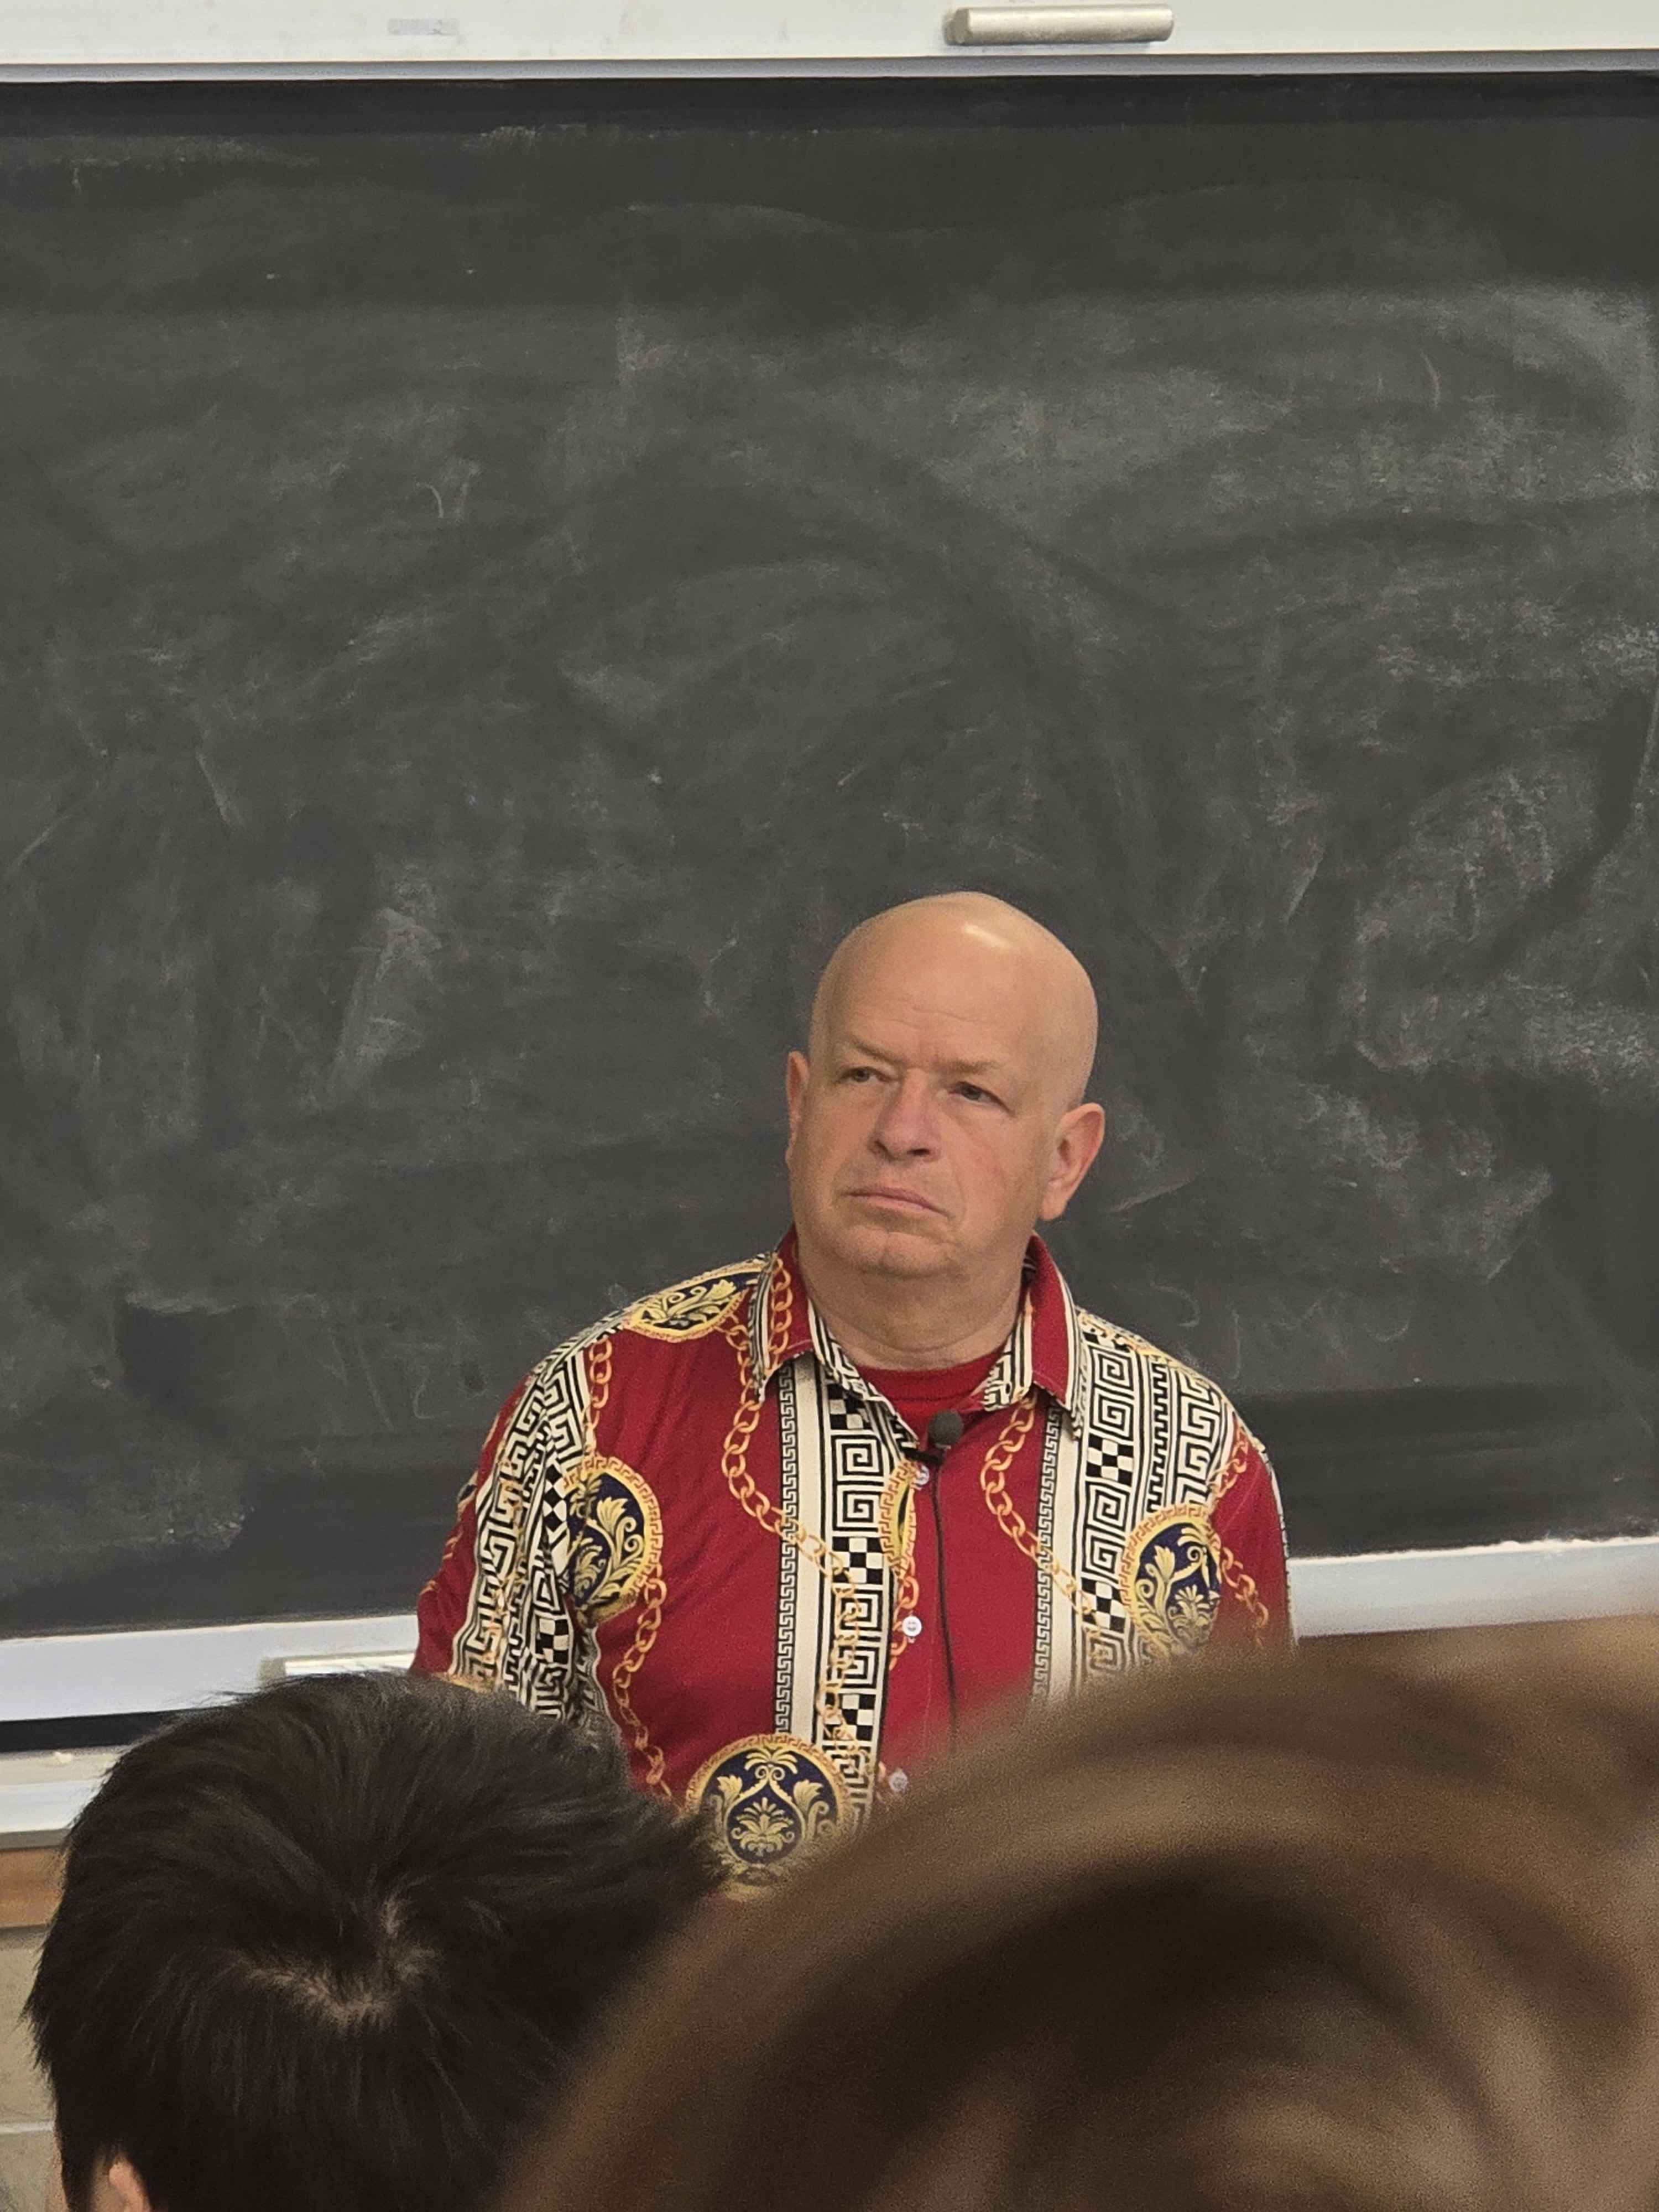
\includegraphics[scale=0.1]{MAT327 Notes/Dror Shirts/dror day 14 shirt.jpg}
\end{figure}

\noindent Recap: $[0, 1]$ is connected, continuous image of connected is connected, and a union of connected sets with a nonempty intersection is connected. This means we have the following theorem,
\begin{simplethm}
    A subset of $\RR$ is connected if and only if it is an interval, i.e.the interval can be open, closed, half-open, etc... whatever, or if it is a ray, such as $(-\infty, a)$, $(-\infty, a]$, etc..., or the whole of $\RR$.
\end{simplethm}
\noindent The theorem is equivalent to saying that if a subset $A \subset \RR$ is convex, if $a, b \in A$ with $a < b$, then $[a, b] \subset A$.
\begin{itemize}
    \item[$(\Leftarrow)$] All of the $9$ cases above are easy. For example,
    \[ (9, \infty) = \bigcup_{n=1}^\infty \left[9 + \frac{1}{n}, n + 20\right]. \]
    \item[$(\Rightarrow)$] If $A$ is not convex, then there exists $a, b, c$ such that $a < c < b$ with $a, b \in A$ but $c \not\in A$. Then $A = (A \cap (-\infty, c)) \cup (A \cup (c, \infty))$. Clearly, both sets in the union are open, so we see this is a separation of $A$. \qed 
\end{itemize}
\begin{simplethm}
    $X, Y \neq \emptyset$ is connected if and only if $X \times Y$ is connected.
\end{simplethm}
\begin{itemize}
    \item[$(\Leftarrow)$] Indeed, $X = \pi_X (X \times Y)$ is a continuous image of connected sets, so it is also connected. We also have $Y = \pi_Y (X \times Y)$, which is also connected. Note that this theorem \textit{isn't} in Munkres because Munkres does not assume $X, Y$ are nonempty.
    \item[$(\Rightarrow)$] Start by observing that $\{x_0\} \times Y$, $X \times \{y_0\}$ is connected. We may pick any arbitrary $x_0, y_0$ in $X, Y$ respectively, so write (we decided to vary on $y_0$ during class)
    \[ X \times Y = \bigcup_{y_0 \in Y} (\{x_0\} \times Y) \cup (X \times \{y_0\}), \]
    which is a union of connected sets with non-empty intersection, i.e. the intersection is $\{x_0\} \times Y$. Note that if either of $X$ or $Y$ are empty, we can simply write the union in terms of the other set. \qed
\end{itemize}

\noindent We now look at some examples. Consider $\RR_\mathrm{box}^\NN$, which is the union of bounded and non-bounded sequences (as seen on the 2010 and 2018 midterms). We know that $\RR_\mathrm{box}^\NN$ is not connected as a result. To check this, observe that all bounded sets $x = \{x_n\}_{n \in \NN}$ are bounded above by $\sup \abs{x_n} \leq M$; then
\[ U_x = \prod_{n = 1}^\infty \left(x_n - 1, x_n + 1\right) \]
is a neighborhood of $x$, while all sequences in $U_x$ are bounded by $M + 1$. By construction, we see that there exists an open neighborhood of bounded sequences about any bounded sequence, so the set is open. Likewise, the set of non-bounded sequences is bounded: we may take $U_x$ as the same construction to see that all sequences in there are unbounded as well. Since the sets of bounded and non-bounded sequences are disjoint, we see that $\RR^\NN$ is not connected in the box topology.
\begin{simplethm}
    For all indices $\alpha$, $X_\alpha$ is connected if and only if $\prod X_\alpha$ is connected in the product topology.\footnote{never saying cylinders again fuck me}
\end{simplethm}
\begin{itemize}
    \item[$(\Leftarrow)$] Same argument as earlier (14.2) literally.
    \item[$(\Rightarrow)$] Intuition: let us fix a point in each $X_\alpha$; then every product of a finite number of spaces and fixed points in the rest of the spaces is connected; taking the union of all these products, we have that its closure is the whole space.
    \medskip\newline
    Pick $x_\alpha \in X_\alpha$ for each $\alpha$; for a finite set $F \subset A$, consider
    \[ B_F = \left\{ y : A \to \bigcup X_\alpha \mid y_\alpha \begin{cases} = x_\alpha & \text{if } \alpha \not\in F \\ \in X_\alpha & \text{otherwise} \end{cases} \right\}. \]
    For each $F$, $B_F \simeq \prod_{\alpha \in F} X_\alpha$ is a finite product of connected space, hence it is connected. Also, $x = (x_\alpha)$ clearly belongs to $B_F$ for every $F$, so the intersection of $B_F$ over all $F$ is clearly nonempty. Thus, the union of all $B_F$ over finite sets $F \subset A$ is connected; for convenience, denote the union as $B$. Then we may write
    \[ B = \bigcup B_F = \left\{ y \in \prod X_\alpha \mid y_\alpha = x_\alpha \text{ for all but finitely many } \alpha \right\}. \]
    We now claim that the closure of $B$ is the full set; $B$ is dense in $\prod X_\alpha$, i.e. $\overline{B} = \prod X_\alpha$, which is equivalent to saying that every non-empty open set in $\prod X_\alpha$ intersects $B$. Indeed, let $U = \prod U_\alpha$ with $U_\alpha = X_\alpha$ almost always be a basic open set in the product $\prod X_\alpha$. Then for $y = (y_\alpha)$, we have that $y_\alpha$ is some element of $U_\alpha$ if $U_\alpha \neq X_\alpha$, and $x_\alpha$ if $U_\alpha$ is the full set. By construction, we see that $y \in B \cap U$. \qed
\end{itemize}
\begin{simplelemma}
    Let $B \subset X$ be connected, and $B \subset A \subset \overline{B}$. Then $A$ is connected.
\end{simplelemma}
\noindent Clearly, the lemma completes the \textit{if} part of the theorem, because $B$ is connected in our case and hence also $\overline{B}$. We now check the lemma. If $C$ is clopen in $A$, then without loss of generality, $C \cap B \neq \emptyset$. Then $C \cap B$ is clopen in $B$, but $B$ is connected, so $C \supset B$. Note that we have $C = \mathrm{cl}_A C$, and we want to compare the closure of $C$ inside $A$ (which is itself) and the closure of $C$ inside $X$. Observe that $\mathrm{cl}_A C = A \cap \mathrm{cl}_X C$, and we have that
\[ A \cap \mathrm{cl}_X C \supset A \cap \mathrm{cl}_X B = A, \]
so $C$ is either trivial, meaning that $A$ has no separation.
\medskip\newline
\noindent We used the fact that $C \subset A \subset X$ implies $\mathrm{cl}_A C = A \cap \mathrm{cl}_X C$ earlier; we prove it now. If $x \in \mathrm{cl}_A C$, then $x \in A$ and every neighborhood of $A$ containing $x$ intersects $C$. This is equivalent to saying that every neighborhood of $x$ in $X$ intersects $C$, which is also equivalent to saying that $x \in \mathrm{cl}_X C$, and we have that $x \in A \cap \mathrm{cl}_X C$. \qed
\medskip\newline
\noindent We now move onto a lighter topic. We say that a set $X$ is \textit{path-connected} if there exists a ``path'' connecting any two points. Formally, for every $a, b \in X$, there exists a continuous function $\gamma : [0, 1] \to X$ such that $\gamma(0) = a, \gamma(1) = b$.
\begin{simplethm}
    If $X$ is path-connected, it is also connected.
\end{simplethm}
\noindent Pick a point $m \in X$, and for every $b \in X$, pick a path, i.e., a continuous function $\gamma_b : [0, 1] \to X$ such that $g_b(0) = m$ and $g_b(1) = b$. Then $S_b = \gamma_b([0, 1])$ is connected with $b \in S_b$ and $m \in S_b$. Now,
\[ \bigcup_{b \in X} S_b = X, \hspace{0.2in} \bigcap S_b \supset \{m\}, \]
meaning this union of $S_b$ is a construction to show that $X$ is connected. Note that the converse is a harder topic we do not talk about yet. \qed
\medskip\newline
We now talk about a few properties.
\begin{enumerate}[label=(\alph*)]
    \item We give an example of a connected, but not path-connected set. The \textit{topologist's since curve} is given by the closure of $S = (-\infty, 0] \times \{0\} \cup \{(x, \sin \frac{1}{x}) \mid x > 0\}$, i.e. $\overline{S} = \{0\} \times [-1, 1] \cup S$.
    \item IVT holds for p.c. spaces.
    \item $[0, 1]$ is p.c.
    \item The continuous image of p.c. is p.c.. Suppose $X$ is p.c., and $f : X \to Y$ is continuous. Then $f(X)$ is also p.c. because the composition of continuous functions is continuous, i.e. $f \circ \gamma_b$ for any $b \in X$ yields a path for $f(m)$ to $f(b)$.
    \item The product, $X = \prod X_\alpha$ is p.c., if and only if for all indices $\alpha$, $X_\alpha$ is also p.c.
    \begin{itemize}
        \item[$(\Rightarrow)$] Writing $X_\alpha = \pi_\alpha (\prod X_\alpha)$, we see that the projection function is continuous, so any path function on $X$ composed with $\pi_\alpha$ yields a path on $X_\alpha$.
        \item[$(\Leftarrow)$] If $X_\alpha$ is p.c., then suppose $x = (x_\alpha)$, $y = (y_\alpha)$ are in $X$. We use the p.c. of each $X_\alpha$ to find a continuous $\gamma_\alpha : [0, 1] \to X_\alpha$ such that $\gamma_\alpha(0) = x_\alpha$ and $\gamma_\alpha(1) = y_\alpha$. Now, consider the combined path $\gamma : [0, 1] \to X$ by $\gamma(t)_\alpha = \gamma_\alpha(t)$ for $t \in [0, 1]$. $\gamma$ is continuous because the second axiom of product spaces states that if a function is continuous in its coordinates (i.e., $\gamma_\alpha$), then the function $\gamma$ itself is continuous. $\gamma(0)$ is clearly $x$, $\gamma(1)$ is clearly $y$, and we are done; we conclude that $X$ is p.c.. \qed
    \end{itemize}
\end{enumerate}

\noindent We end class with a riddle: do there exist disjoint connected paths $A, B$ on $[0, 1] \times [0, 1]$ such that $A$ goes from $(0, 0)$ to $(1, 1)$ and $B$ goes from $(1, 0)$ to $(0, 1)$ in the standard topology?